\chapter{Katalisis}\label{ch:g12:catalysis}

Sebotol larutan hidrogen peroksida tersimpan di lemari kamar mandi
selama berbulan-bulan tanpa berubah. Jika dituangkan pada lutut yang
lecet, larutan itu langsung berbuih: sesuatu di dalam darah membuatnya
terurai dalam beberapa detik menjadi air dan oksigen. Sesuatu itu tidak
habis terpakai, dan tidak muncul dalam \omterm{def:g8:balanced-equations:equation}{persamaan reaksinya}. Itulah
\omterm{def:g12:catalysis:catalyst}{katalis}. \omterm{def:g12:catalysis:catalyst}{Katalis} memungkinkan sebagian besar industri kimia,
membersihkan gas buang mobil, dan menjalankan setiap reaksi kehidupan.

\begin{recall}
Laju sebuah reaksi dan faktor-faktor kinetik yang mengubahnya
(\cref{ch:g12:reaction-rates}). Mekanisme adalah rangkaian \omterm{def:g12:curly-arrows:mechanism}{tahap
elementer}, melalui zat-zat antara (\cref{ch:g12:curly-arrows}).
\end{recall}

\section{Apa itu katalis}

\begin{definition}[Katalis, katalisis]\label{def:g12:catalysis:catalyst}
Yang disebut \emph{katalis}\index{katalis} adalah spesies yang
mempercepat sebuah reaksi tanpa habis terpakai: katalis ikut serta
dalam mekanisme tetapi dikembalikan, tanpa berubah, pada akhirnya, dan
tidak muncul dalam persamaan keseluruhan. Percepatan reaksi oleh katalis
disebut \emph{katalisis}\index{katalisis}.
\end{definition}

\begin{proposition}[Katalis mengubah jalan, bukan tujuan]\label{prop:g12:catalysis:path}
\omterm{def:g12:catalysis:catalyst}{Katalis} membuka mekanisme lain, yang penghalang energinya lebih rendah
daripada penghalang reaksi tanpa \omterm{def:g12:catalysis:catalyst}{katalis}, sehingga lebih banyak
pertemuan antarpartikel yang berhasil. \omterm{def:g12:catalysis:catalyst}{Katalis} tidak mengubah produk
yang terbentuk, tidak pula \omterm{def:g10:reaction-progress-table:system}{keadaan akhir} yang dicapai; \omterm{def:g12:catalysis:catalyst}{katalis} hanya
mencapainya lebih cepat.
\end{proposition}

\begin{proof}
Diterima tanpa bukti: profil energinya dipelajari dalam buku Tahun
Pertama universitas. Bahwa \omterm{def:g10:reaction-progress-table:system}{keadaan akhirnya} tidak berubah merupakan
akibat dari dikembalikannya \omterm{def:g12:catalysis:catalyst}{katalis}: reaksi keseluruhannya, \omterm{def:g7:chemical-reactions:reactant}{pereaksi} dan
produknya, tetap sama.
\end{proof}

\begin{omfigure}
\begin{minipage}{0.49\linewidth}
\begin{tikzpicture}
\begin{axis}[width=\linewidth, height=5.4cm, xmin=0, xmax=1, ymin=-60,
    ymax=110, xtick=\empty, ytick=\empty, axis lines*=left,
    xlabel={kemajuan reaksi}, ylabel={energi},
    label style={font=\small}, legend style={font=\scriptsize,
    at={(0.02,0.99)}, anchor=north west, draw=none}, legend cell align=left]
  \addplot[very thick, omDef] table[x=s, y=Eu] {figdata/out/grade-12-catalysis-a.dat};
  \addplot[very thick, omProp] table[x=s, y=Ec] {figdata/out/grade-12-catalysis-a.dat};
  \legend{tanpa katalis, dengan katalis}
  \node[font=\scriptsize, anchor=north west] at (axis cs:0.02,-4) {pereaksi};
  \node[font=\scriptsize, anchor=south east] at (axis cs:0.99,-36) {produk};
\end{axis}
\end{tikzpicture}
\end{minipage}\hfill
\begin{minipage}{0.49\linewidth}
\begin{tikzpicture}
\begin{axis}[width=\linewidth, height=5.4cm, xmin=0, xmax=60, ymin=0,
    ymax=80, xlabel={$t$ (\si{min})}, ylabel={\ce{O2} yang dilepaskan (\si{mL})},
    axis lines*=left, ymajorgrids, grid style={gray!20},
    tick label style={font=\scriptsize}, label style={font=\small},
    legend style={font=\scriptsize, at={(0.98,0.03)}, anchor=south east,
    draw=none}, legend cell align=left]
  \addplot[very thick, omDef] table[x=t, y=Vu] {figdata/out/grade-12-catalysis-b.dat};
  \addplot[very thick, omProp] table[x=t, y=Vc] {figdata/out/grade-12-catalysis-b.dat};
  \legend{tanpa katalis, dengan katalis}
\end{axis}
\end{tikzpicture}
\end{minipage}

{\small Kiri: energi sepanjang jalannya reaksi; jalan dengan \omterm{def:g12:catalysis:catalyst}{katalis}
melewati sebuah zat antara dan dua penghalang yang lebih rendah. Kanan:
oksigen yang dilepaskan larutan hidrogen peroksida; \omterm{def:g12:catalysis:catalyst}{katalis} mempercepat
reaksinya, tetapi volume akhirnya sama. (Kurva model.)}
\end{omfigure}

\section{Katalisis homogen}

\begin{definition}[Katalisis homogen dan heterogen]\label{def:g12:catalysis:homogeneous}
\omterm{def:g12:catalysis:catalyst}{Katalisisnya} disebut \emph{katalisis homogen}\index{katalisis homogen}
jika \omterm{def:g12:catalysis:catalyst}{katalis} berada dalam fase yang sama dengan \omterm{def:g7:chemical-reactions:reactant}{pereaksi} (misalnya
terlarut bersama \omterm{def:g7:chemical-reactions:reactant}{pereaksi}), dan \emph{katalisis
heterogen}\index{katalisis heterogen} jika \omterm{def:g12:catalysis:catalyst}{katalis} berada dalam fase
lain, biasanya berupa padatan yang permukaannya dicapai \omterm{def:g7:chemical-reactions:reactant}{pereaksi} dari
gas atau cairan.
\end{definition}

\begin{example}[Ion iodida dan hidrogen peroksida]\label{ex:g12:catalysis:iodide}
Hidrogen peroksida dengan sendirinya terurai sangat lambat:
\ce{2H2O2 -> 2H2O + O2}. Jika sedikit kalium iodida dilarutkan di
dalamnya, larutan itu langsung berbuih. \omterm{def:g9:ions:ion}{Ion} iodida membuka jalan dalam
dua tahap:
\[
  \ce{H2O2 + I- -> H2O + IO-}, \qquad
  \ce{H2O2 + IO- -> H2O + O2 + I-} .
\]
Jika dijumlahkan, kedua tahap itu kembali memberikan
\ce{2H2O2 -> 2H2O + O2}: \omterm{def:g9:ions:ion}{ion} iodida, yang dipakai pada tahap pertama dan
dikembalikan pada tahap kedua, adalah \omterm{def:g12:catalysis:catalyst}{katalisnya}; \omterm{def:g9:ions:ion}{ion} \ce{IO-} adalah
zat antara.
\end{example}


\begin{example}[Ion besi(III)]\label{ex:g12:catalysis:iron}
\omterm{def:g9:ions:ion}{Ion} besi(III) juga mengatalisis penguraian itu, melalui pasangan
\ce{Fe^{3+}}/\ce{Fe^{2+}} (\cref{ch:g11:redox}): mula-mula \omterm{def:g9:ions:ion}{ion} itu
mengoksidasi hidrogen peroksida,
\ce{2Fe^{3+} + H2O2 -> 2Fe^{2+} + O2 + 2H+}, lalu \omterm{def:g9:ions:ion}{ion-ion} besi(II) yang
terbentuk dioksidasi kembali oleh hidrogen peroksida yang lain,
\ce{2Fe^{2+} + H2O2 + 2H+ -> 2Fe^{3+} + 2H2O}. Warna jingga pucat
larutan berubah kehijauan selama gas dilepaskan, lalu kembali ketika
hidrogen peroksida habis: tanda bahwa \omterm{def:g12:catalysis:catalyst}{katalis} ikut serta dan
diregenerasi.
\end{example}

\section{Katalisis heterogen}

Banyak \omterm{def:g12:catalysis:catalyst}{katalis} industri berupa padatan: \omterm{def:g9:periodic-table-first-look:metal}{logam} seperti platina,
paladium, nikel, atau besi, atau oksida. Reaksinya berlangsung di
permukaan \omterm{def:g12:catalysis:catalyst}{katalis}, dalam tiga tahap: \omterm{def:g7:atoms-and-molecules:molecule}{molekul-molekul} \omterm{def:g7:chemical-reactions:reactant}{pereaksi} ditahan
di permukaan (teradsorpsi), tempat ikatan-ikatannya melemah; \omterm{def:g7:atoms-and-molecules:molecule}{molekul} itu
bereaksi di sana; produk-produknya meninggalkan permukaan, yang menjadi
bebas untuk \omterm{def:g7:atoms-and-molecules:molecule}{molekul-molekul} baru. Karena itu \omterm{def:g12:catalysis:catalyst}{katalis} dibuat dengan
permukaan seluas mungkin: serbuk halus, atau lapisan tipis pada
penyangga berpori.

\begin{omfigure}
\begin{tikzpicture}[font=\small]
  \foreach \x in {0,4.2,8.4} {
    \fill[black!25] (\x,0) rectangle (\x+3.4,0.35);
    \foreach \i in {0,1,2,3,4,5,6,7} \shade[ball color=black!35] (\x+0.21+\i*0.425,0.35) circle (0.2);
  }
  % 1. adsorption
  \node[aH, minimum size=3.2mm] at (0.9,0.75) {};
  \node[aH, minimum size=3.2mm] at (1.3,0.75) {};
  \node[aH, minimum size=3.2mm] (h1) at (2.2,1.8) {};
  \node[aH, minimum size=3.2mm] (h2) at (2.6,1.8) {};
  \draw[bond, line width=1.2pt] (h1.east) -- (h2.west);
  \draw[->, omProp, thick] (2.4,1.55) -- (2.0,1.0);
  \node[anchor=north, align=center] at (1.7,-0.1) {1. teradsorpsi:\\ ikatan \ce{H-H} putus};
  % 2. reaction on the surface
  \node[aC] (c1) at (5.5,1.05) {}; \node[aC] (c2) at (6.2,1.05) {};
  \draw[bond, line width=1.4pt] (c1) -- (c2);
  \node[aH, minimum size=3.2mm] at (5.3,0.75) {};
  \node[aH, minimum size=3.2mm] at (6.6,0.75) {};
  \node[anchor=north, align=center] at (5.9,-0.1) {2. atom H bergabung\\ dengan molekul\\ teradsorpsi};
  % 3. desorption
  \node[aC] (c3) at (9.6,1.8) {}; \node[aC] (c4) at (10.3,1.8) {};
  \draw[bond, line width=1.4pt] (c3) -- (c4);
  \foreach \a/\c in {150/c3,210/c3,90/c3,30/c4,-30/c4,90/c4}
    \node[aH, minimum size=2.8mm] at ($(\c)+(\a:0.42)$) {};
  \draw[->, omProp, thick] (11.0,1.2) -- (11.0,2.2);
  \node[anchor=north, align=center] at (10.1,-0.1) {3. produk\\ meninggalkan\\ permukaan};
\end{tikzpicture}

{\small \omterm{def:g12:curly-arrows:categories}{Adisi} hidrogen pada etena di permukaan \omterm{def:g9:periodic-table-first-look:metal}{logam}: adsorpsi, reaksi,
desorpsi. \omterm{def:g9:periodic-table-first-look:metal}{Logamnya} dikembalikan tanpa berubah.}
\end{omfigure}

\begin{example}[Konverter katalitik]\label{ex:g12:catalysis:converter}
Gas buang mesin bensin mengandung karbon monoksida dan nitrogen
monoksida, keduanya beracun, serta \omterm{def:g4:what-a-fire-needs:fuel}{bahan bakar} yang tidak \omterm{def:g4:what-a-fire-needs:burning}{terbakar}. Di
dalam konverter katalitik, sebuah sarang lebah keramik yang dilapisi
platina dan rodium, gas-gas itu bereaksi di permukaan \omterm{def:g9:periodic-table-first-look:metal}{logam}:
\[
  \ce{2CO + 2NO -> 2CO2 + N2} ,
\]
dan hidrokarbonnya \omterm{def:g4:what-a-fire-needs:burning}{terbakar} menjadi karbon dioksida dan air. Gas-gas
itu melintasi konverter dalam sepersekian detik, terlalu cepat bagi
reaksi apa pun tanpa \omterm{def:g12:catalysis:catalyst}{katalis}.
\end{example}

\begin{omfigure}
\begin{tikzpicture}[font=\small]
  \fill[black!12, draw=black!60, rounded corners=6pt] (0,0) rectangle (6,2.4);
  \foreach \x in {0.3,0.6,0.9,1.2,1.5,1.8,2.1,2.4,2.7,3.0,3.3,3.6,3.9,4.2,4.5,4.8,5.1,5.4,5.7} \draw[black!35] (\x,0.2) -- (\x,2.2);
  \foreach \y in {0.5,0.9,1.3,1.7,2.1} \draw[black!35] (0.2,\y) -- (5.8,\y);
  \fill[black!40] (-1.4,0.9) rectangle (0,1.5);
  \fill[black!40] (6,0.9) rectangle (7.4,1.5);
  \draw[->, very thick, omThm] (-2.6,1.2) -- (-1.5,1.2);
  \node[anchor=east, align=right, omThm] at (-2.7,1.2) {\ce{CO}, \ce{NO},\\ hidrokarbon};
  \draw[->, very thick, omMeth] (7.5,1.2) -- (8.6,1.2);
  \node[anchor=west, align=left, omMeth] at (8.7,1.2) {\ce{CO2}, \ce{N2},\\ \ce{H2O}};
  \node[align=center, fill=white, inner sep=2pt] at (3,1.2) {sarang lebah keramik\\ berlapis Pt dan Rh};
\end{tikzpicture}

{\small Konverter katalitik, dipotong memanjang: ribuan saluran tipis
memberi gas buang permukaan berlapis \omterm{def:g9:periodic-table-first-look:metal}{logam} yang sangat luas.}
\end{omfigure}

\begin{omfigure}
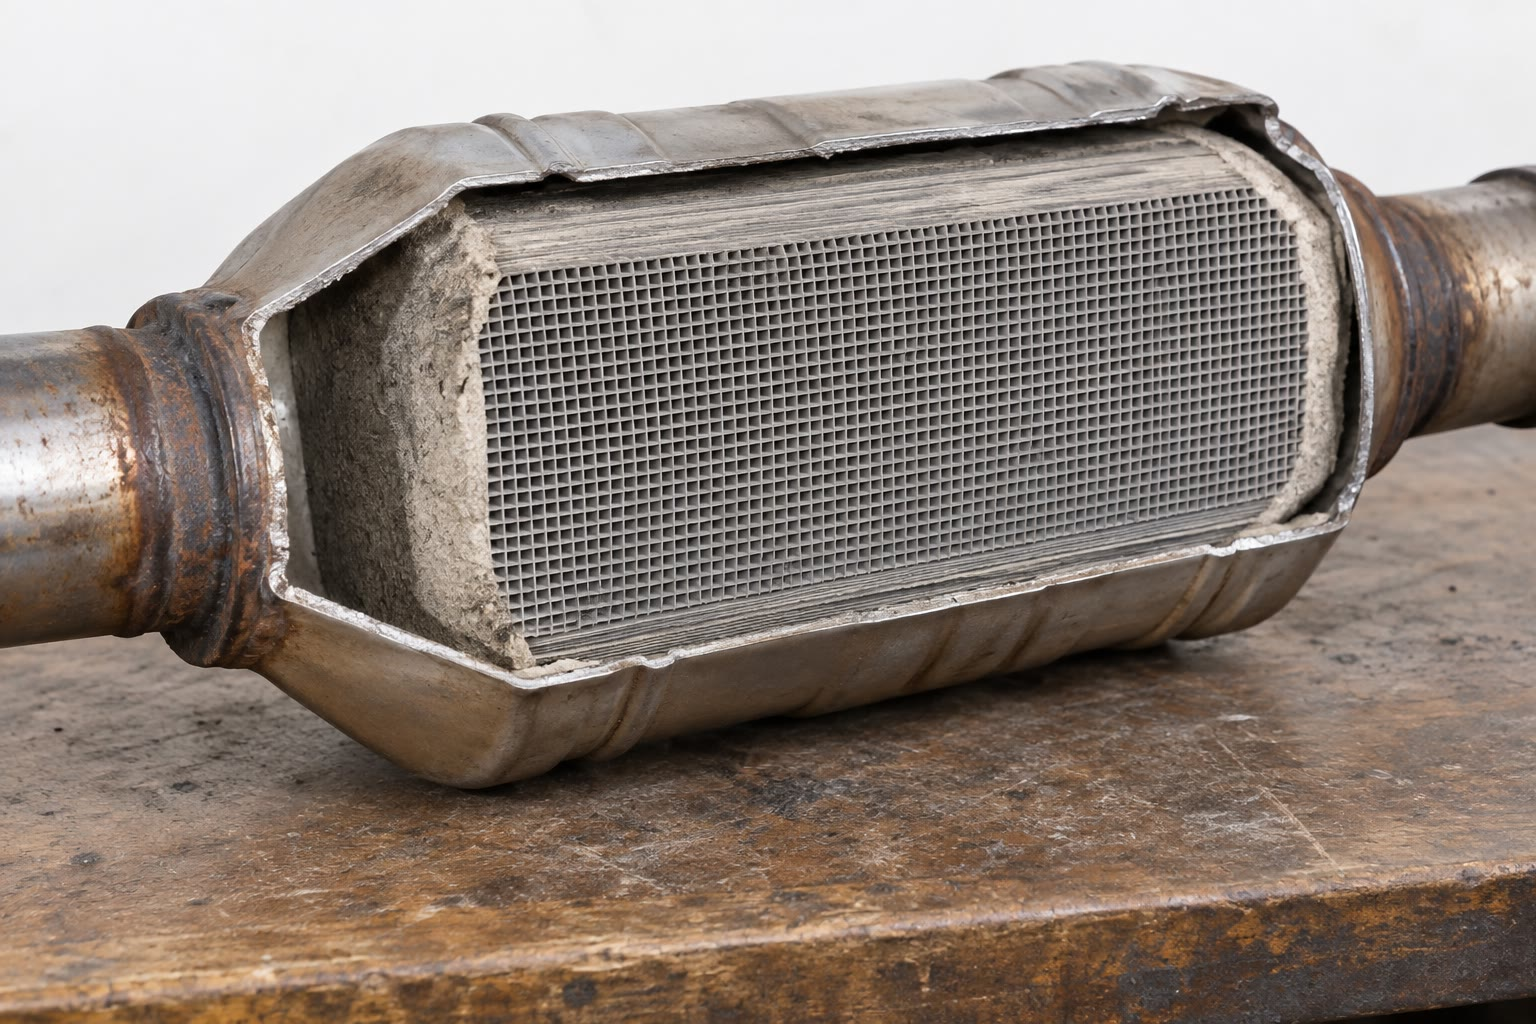
\includegraphics[width=0.45\linewidth]{images/book1/ai/g12-catalytic-converter.jpg}

{\small Konverter katalitik yang dibelah: inti sarang lebahnya.}
\end{omfigure}

\begin{history}[Haber, Bosch, dan amonia]
% ledger: haber:T, haber:p, nh3:world-2024
Pada awal abad kedua puluh, ahli kimia Fritz Haber menemukan cara
menggabungkan nitrogen \omterm{def:g4:air-a-mixture-of-gases:air}{udara} dengan hidrogen,
\ce{N2 + 3H2 -> 2NH3}, dengan \omterm{def:g12:catalysis:catalyst}{katalis} berbasis besi, dan insinyur Carl
Bosch mengubahnya menjadi proses industri. Proses itu masih berjalan
hingga kini pada 400 sampai \qty{500}{\celsius} dan 150 sampai
\qty{250}{atm}. Pada tahun 2024 dunia membuat amonia yang mengandung
sekitar 150 juta ton nitrogen, sebagian besar untuk pupuk: sebagian
besar nitrogen dalam makanan kita pernah melewati \omterm{def:g12:catalysis:catalyst}{katalis} semacam itu.
\end{history}

\section{Enzim}

\begin{definition}[Enzim]\label{def:g12:catalysis:enzyme}
Yang disebut \emph{enzim}\index{enzim} adalah protein yang dibuat oleh
makhluk hidup dan mengatalisis satu reaksi dalam kimia tubuhnya. Enzim
sangat efisien dan sangat spesifik: masing-masing hanya cocok dengan
beberapa \omterm{def:g7:atoms-and-molecules:molecule}{molekul}, dan enzim bekerja paling baik dalam rentang suhu dan
keasaman yang sempit.
\end{definition}

\begin{example}[Katalase]\label{ex:g12:catalysis:catalase}
Hidrogen peroksida terbentuk di dalam sel sebagai hasil samping, dan
berbahaya bagi sel. \omterm{def:g12:catalysis:enzyme}{Enzim} katalase, yang terdapat dalam darah, hati, dan
banyak jaringan tumbuhan, menguraikannya menjadi air dan oksigen dengan
kecepatan yang luar biasa: itulah buih pada lutut yang lecet, atau pada
irisan kentang mentah. Kentang rebus tidak menghasilkan buih: pemanasan
telah merusak bentuk \omterm{def:g12:catalysis:enzyme}{enzimnya}.
\end{example}

\begin{omfigure}
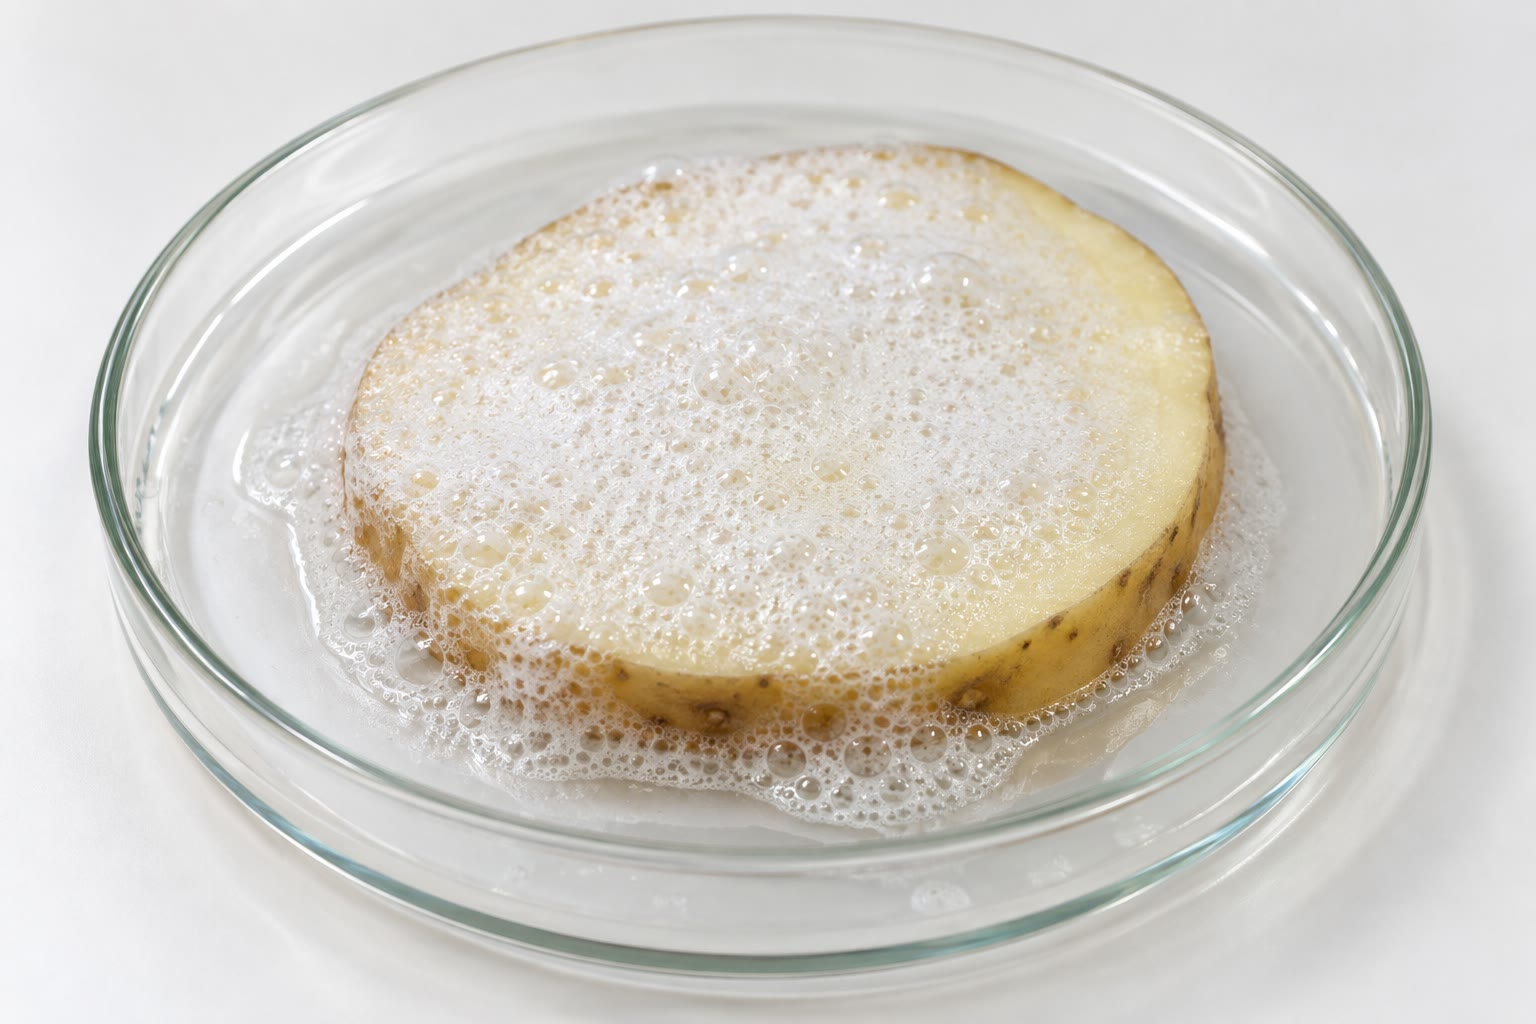
\includegraphics[width=0.45\linewidth]{images/book1/ai/g12-potato-peroxide.jpg}

{\small Hidrogen peroksida pada irisan kentang mentah: katalase sedang
bekerja.}
\end{omfigure}

\section{Selektivitas}

\begin{definition}[Katalis selektif]\label{def:g12:catalysis:selective}
Jika \omterm{def:g7:chemical-reactions:reactant}{pereaksi} yang sama dapat menjalani beberapa reaksi, sebuah
\emph{katalis selektif}\index{katalis selektif} mempercepat salah
satunya jauh lebih banyak daripada yang lain, sehingga menentukan
produk mana yang terbentuk.
\end{definition}

\begin{example}[Dua nasib etanol]\label{ex:g12:catalysis:ethanol}
Uap etanol panas yang dialirkan di atas alumina kehilangan air dan
menghasilkan etena, \ce{C2H5OH -> C2H4 + H2O} (sebuah \omterm{def:g12:curly-arrows:categories}{eliminasi}); jika
dialirkan di atas tembaga panas, uap itu kehilangan hidrogen dan
menghasilkan etanal, \ce{C2H5OH -> CH3CHO + H2}. \omterm{def:g7:chemical-reactions:reactant}{Pereaksi} sama, dua
\omterm{def:g12:catalysis:catalyst}{katalis}, dua produk.
\end{example}

\begin{remark}[Industri dan kehidupan berjalan dengan katalis]\label{rem:g12:catalysis:everywhere}
Sebagian besar produk industri kimia, dari \omterm{def:g4:what-a-fire-needs:fuel}{bahan bakar} sampai \omterm{def:g8:plastics:plastic}{plastik}
dan pupuk, dibuat dengan \omterm{def:g12:catalysis:catalyst}{katalis}; menemukan \omterm{def:g12:catalysis:catalyst}{katalis} yang lebih aktif
atau lebih selektif menghemat energi dan mengurangi limbah. Setiap
reaksi dalam sel hidup dikatalisis oleh sebuah \omterm{def:g12:catalysis:enzyme}{enzim}.
\end{remark}

\begin{safety}{\ghs[0.82cm]{GHS03}\ghs[0.82cm]{GHS05}\ghs[0.82cm]{GHS07}}
% ledger: ghs:H2O2
Hidrogen peroksida pekat adalah \omterm{def:g11:redox:oxidant}{oksidator} kuat yang dapat memperbesar
api, membakar kulit dan mata, serta berbahaya jika tertelan. Larutan
encer di laboratorium tetap memerlukan kacamata pelindung dan sarung
tangan; penguraiannya melepaskan oksigen, sehingga tidak pernah
dilakukan di dalam wadah tertutup.
\end{safety}

\section{Latihan}


\begin{exercise}[$\star$]\label{exo:g12:catalysis:1}
Pada penguraian hidrogen peroksida yang dikatalisis \omterm{def:g9:ions:ion}{ion} iodida, spesies
mana yang menjadi \omterm{def:g7:chemical-reactions:reactant}{pereaksi}, mana yang menjadi produk, mana yang menjadi
\omterm{def:g12:catalysis:catalyst}{katalis}, dan mana yang menjadi zat antara?
\end{exercise}

\begin{exercise}[$\star$]\label{exo:g12:catalysis:2}
\omterm{def:g12:catalysis:homogeneous}{Katalisis homogen} atau heterogen: \omterm{def:g9:ions:ion}{ion} iodida dalam larutan hidrogen
peroksida; platina dalam konverter katalitik; besi dalam \omterm{def:g10:synthesis-yield:synthesis}{sintesis}
amonia; \omterm{def:g9:ions:ion}{ion} besi(III) dalam larutan hidrogen peroksida?
\end{exercise}

\begin{exercise}[$\star$]\label{exo:g12:catalysis:3}
Pada profil energi, jalan mana yang memiliki penghalang lebih tinggi?
Apakah energi awal dan energi akhirnya sama pada kedua jalan? Apa
artinya bagi produknya?
\end{exercise}

\begin{exercise}[$\star$]\label{exo:g12:catalysis:4}
Mengapa \omterm{def:g12:catalysis:catalyst}{katalis} tidak muncul dalam persamaan keseluruhan sebuah reaksi?
\end{exercise}

\begin{exercise}[$\star$]\label{exo:g12:catalysis:5}
Mengapa \omterm{def:g12:catalysis:catalyst}{katalis} padat di industri dipakai sebagai serbuk halus atau
sebagai lapisan tipis pada penyangga berpori?
\end{exercise}

\begin{exercise}[$\star\star$]\label{exo:g12:catalysis:6}
Jumlahkan kedua tahap penguraian hidrogen peroksida yang dikatalisis
besi(III), lalu tunjukkan bahwa \omterm{def:g9:ions:ion}{ion-ion} besi dan \omterm{def:g9:ions:ion}{ion-ion} hidrogen saling
meniadakan.
\end{exercise}

\begin{exercise}[$\star\star$]\label{exo:g12:catalysis:7}
Bacalah kurva oksigen yang dilepaskan. Berapa lama waktu yang
diperlukan setiap percobaan untuk melepaskan setengah volume akhirnya?
Dengan faktor berapa \omterm{def:g12:catalysis:catalyst}{katalis} memperpendek waktu itu?
\end{exercise}

\begin{exercise}[$\star\star$]\label{exo:g12:catalysis:8}
Bensin bertimbal tidak dipakai pada mobil yang dilengkapi konverter
katalitik: timbal mengendap pada platina dan tetap di sana. Jelaskan
mengapa hal ini merusak konverter, walaupun platina tidak habis terpakai
oleh reaksi yang normal.
\end{exercise}

\begin{exercise}[$\star\star$]\label{exo:g12:catalysis:9}
Seorang siswa mengukur buih yang dihasilkan irisan kentang dalam
hidrogen peroksida pada 10, 25, 37, 60, dan \qty{80}{\celsius}: buihnya
bertambah sampai sekitar \qty{37}{\celsius}, lalu berkurang, dan hampir
hilang pada \qty{80}{\celsius}. Jelaskan kedua bagian kurva itu.
\end{exercise}

\begin{exercise}[$\star\star$]\label{exo:g12:catalysis:10}
Tuliskan \omterm{def:g8:balanced-equations:equation}{persamaan reaksi} di dalam konverter katalitik antara karbon
monoksida dan nitrogen monoksida, lalu periksalah bahwa persamaan itu
setara. Mengapa kedua polutan itu tersingkir sekaligus?
\end{exercise}

\begin{exercise}[$\star\star$]\label{exo:g12:catalysis:11}
Sebanyak \qty{10.0}{mL} larutan hidrogen peroksida melepaskan
\qty{72}{mL} oksigen pada \qty{20}{\celsius} jika terurai seluruhnya.
Hitung jumlah oksigennya ($V_m = \qty{24.1}{L/mol}$), lalu konsentrasi
hidrogen peroksida dalam larutan itu.
\end{exercise}

\begin{exercise}[$\star\star\star$]\label{exo:g12:catalysis:12}
Uap etanol yang dialirkan di atas alumina menghasilkan etena; di atas
tembaga, uap itu menghasilkan etanal. Tuliskan kedua persamaannya,
sebutkan kategori reaksi yang pertama, lalu jelaskan apa itu \omterm{def:g12:catalysis:selective}{katalis
selektif}.
\end{exercise}

\begin{exercise}[$\star\star\star$]\label{exo:g12:catalysis:13}
Sebuah \omterm{def:g12:catalysis:catalyst}{katalis} membuat reaksi sepuluh kali lebih cepat. Seorang siswa
mengatakan bahwa \omterm{def:g12:catalysis:catalyst}{katalis} itu juga menghasilkan produk sepuluh kali lebih
banyak. Perbaikilah pernyataan itu, dengan memakai kurva oksigen yang
dilepaskan.
\end{exercise}

\begin{exercise}[$\star\star\star$]\label{exo:g12:catalysis:14}
Satu \omterm{def:g7:atoms-and-molecules:molecule}{molekul} katalase menguraikan sekitar beberapa juta \omterm{def:g7:atoms-and-molecules:molecule}{molekul}
hidrogen peroksida per detik. Dengan mengambil $\num{5e6}$ per detik,
berapa lama waktu yang diperlukan satu \omterm{def:g7:atoms-and-molecules:molecule}{molekul} \omterm{def:g12:catalysis:enzyme}{enzim} untuk menguraikan
satu \omterm{def:g10:the-mole:amount}{mol} hidrogen peroksida? Berapa \omterm{def:g7:atoms-and-molecules:molecule}{molekul} \omterm{def:g12:catalysis:enzyme}{enzim} yang akan
menyelesaikannya dalam satu detik? (Perhitungan orde besar; lajunya
adalah data latihan.)
\end{exercise}

\begin{exercise}[$\star\star\star$]\label{exo:g12:catalysis:15}
% ledger: nh3:world-2024
Pada tahun 2024 dunia membuat sekitar 150 juta ton nitrogen dalam bentuk
amonia. Berapa massa amonia itu? Berapa jumlah gas nitrogen yang
digabungkan?
\end{exercise}

\section{Soal: Hidrogen Peroksida Penata Rambut}

\begin{problem}[{Soal akhir pekan --- berapa konsentrasi hidrogen
peroksida ``20 volume''?}]
\label{pb:g12:catalysis:1}
% ledger: const:Vm1, ghs:H2O2, aw:H, aw:O
Penata rambut memakai larutan hidrogen peroksida yang diberi label
dalam ``volume'': larutan ``20 volume'' adalah larutan yang
\qty{1}{L}-nya melepaskan \qty{20}{L} oksigen jika terurai seluruhnya,
dengan gas yang diukur pada \qty{0}{\celsius} dan tekanan atmosfer
normal, tempat satu \omterm{def:g10:the-mole:amount}{mol} gas menempati \qty{22.4}{L}.

\medskip
\noindent\textbf{Bagian I --- Penguraiannya.}
\begin{enumerate}
  \item Tuliskan persamaan penguraian hidrogen peroksida.
  \item Apakah penguraian itu \omterm{def:g11:redox:reaction}{reaksi redoks}? Tentukan \omterm{def:g11:redox:oxidant}{oksidator} dan
        \omterm{def:g11:redox:oxidant}{reduktornya} (hidrogen peroksida adalah keduanya).
  \item Mengapa sebotol larutan itu tahan berbulan-bulan, padahal
        reaksinya mungkin terjadi?
\end{enumerate}

\medskip
\noindent\textbf{Bagian II --- Arti ``20 volume''.}
\begin{enumerate}[resume]
  \item Berapa jumlah oksigen yang dilepaskan \qty{1}{L} larutan itu?
  \item Simpulkan jumlah hidrogen peroksida dalam \qty{1}{L}.
  \item Berikan \omterm{def:g10:concentration-and-dilution:molar-concentration}{konsentrasi molarnya}.
  \item Hitung \omterm{def:g10:the-mole:molar-mass}{massa molar} hidrogen peroksida dan \omterm{def:g10:concentration-and-dilution:mass-concentration}{konsentrasi massanya}.
  \item Apa arti ``10 volume'' dalam \omterm{def:g10:the-mole:amount}{mol} per liter?
\end{enumerate}

\medskip
\noindent\textbf{Bagian III --- Dua \omterm{def:g12:catalysis:catalyst}{katalis}.}
\begin{enumerate}[resume]
  \item Setetes darah (katalase) dan beberapa tetes besi(III) klorida
        masing-masing ditambahkan pada sebuah sampel. \omterm{def:g12:catalysis:catalyst}{Katalisis} apa
        masing-masing?
  \item Tuliskan kedua tahap \omterm{def:g12:catalysis:catalyst}{katalisis} besi(III), lalu periksalah bahwa
        jumlahnya adalah reaksi penguraian itu.
  \item Dengan kurva oksigen yang dilepaskan, uraikan bagaimana volume
        oksigen berubah dengan dan tanpa \omterm{def:g12:catalysis:catalyst}{katalis}, dan apa yang tetap
        sama.
  \item Mengapa warna sampel yang dikatalisis besi(III) berubah selama
        reaksi lalu kembali pada akhirnya?
  \item Mengapa kentang rebus tidak membuat larutan itu berbuih?
\end{enumerate}

\medskip
\noindent\textbf{Bagian IV --- Botolnya.}
\begin{enumerate}[resume]
  \item Berapa volume oksigen, yang diukur pada \qty{0}{\celsius}, yang
        dapat dilepaskan sebotol \qty{100}{mL}?
  \item Berapa volume itu pada \qty{20}{\celsius} ($V_m =
        \qty{24.1}{L/mol}$)?
  \item Mengapa tutup botol semacam itu harus membiarkan gas keluar
        perlahan-lahan?
  \item Sebuah botol yang telah lama disimpan dititrasi dan ternyata
        mengandung \qty{1.50}{mol/L}. Berapa ``volume'' larutan itu
        sekarang?
  \item Berapa bagian hidrogen peroksida yang telah terurai?
  \item Nyatakan jawaban akhirnya: berapa \omterm{def:g10:concentration-and-dilution:molar-concentration}{konsentrasi molar} larutan
        hidrogen peroksida ``20 volume''?
\end{enumerate}
\end{problem}
